\documentclass[12pt]{article}

\usepackage{sbc-template}

\usepackage{graphicx,url}

%\usepackage[brazil]{babel}
\usepackage[utf8]{inputenc}

\usepackage{amsmath}
\usepackage{listings}
\usepackage{xspace}
\usepackage{hyperref}  % Enables \autoref
\usepackage{tabularx}
\usepackage[table]{xcolor}
\usepackage{caption}
\usepackage{subcaption}
% \setlength\extrarowheight{2pt} % make the tables look less cramped

\usepackage{tikz}
\usetikzlibrary{shapes.misc, shapes.symbols, fit, positioning, quotes}

\usepackage[inline]{enumitem} % inline lists


\usepackage{tcolorbox}
\usepackage{soul}
\sethlcolor{red}
\newcommand{\mycommentbox}[1]{%
  \begin{tcolorbox}[colback=red!20!white,colframe=red,title=Comment]
      #1
  \end{tcolorbox}
}
\newcommand{\mycomment}[1]{%
	\hl{#1}
}

\newlist{inlinelist}{enumerate*}{1}
\setlist[inlinelist]{label=(\roman*)}



\newcommand{\pathsec}{\textbf{PathSec}\xspace}
\newcommand{\nodeid}{\texttt{node\_id}\xspace}
\newcommand{\nodeids}{\texttt{node\_id}s\xspace}
\newcommand{\portid}{\texttt{port\_id}\xspace}
\newcommand{\portids}{\texttt{port\_id}s\xspace}
\newcommand{\routeid}{\texttt{route\_id}\xspace}
\newcommand{\routeids}{\texttt{route\_id}s\xspace}
\newcommand{\timestamp}{\texttt{timestamp}\xspace}
\newcommand{\lhash}{\texttt{l\_hash}\xspace}
\newcommand{\nhop}{\texttt{nhop}\xspace}
\newcommand{\polka}{\textit{PolKA}\xspace}
\newcommand{\pIV}{\textit{P4}\xspace}
\newcommand{\bmv}{\textit{BMv2}\xspace}
\newcommand{\siphash}{\textit{HalfSipHash}\xspace}


\sloppy

\title{Implementing and Testing a Probing-Based Path Verification for PolKA Source Routing Protocol}

\author{Henrique C. Layber, Roberta L. Gomes, Magnos Martinello}


\address{Department of Informatics\\Federal University of Espírito Santo (UFES) -- Vitória, ES -- Brazil
  \email{henrique.layber@edu.ufes.br,\{roberta.gomes, magnos.martinello\}@ufes.br}
}



\begin{document} 

\maketitle

\begin{abstract}
\end{abstract}
     
\begin{resumo} 
  Este trabalho apresenta uma implementação prova-de-conceito e testes do \pathsec\cite{pathsec}, um mecanismo de sondagem e verificação de rota para o protocolo de roteamento na origem \polka. O mecanismo é baseado em uma combinação de funções hash, calculadas por switches de núcleo sem estado, e permitem uma parte confiável verificar se um pacote percorreu a rede ao longo do caminho definido pela origem. A implementação foi feita no Mininet usando BMv2 programados em P4.
\end{resumo}

{\footnotesize\textbf{Keywords -- Path Aware; Network Security; Path Verification; In-networking Programming}}


% Probing
\section{Introduction}
% O que foi feito
% Motivaçao (!!)
% Oq é SR e Probe-Based Verification (PBV)

% - motivação source routing
% - com isso, há a proposta do polka (sistema de resíduos sem explicar o que é precisamente)
% - mas que que há uma limitação: como comprovar que de fato a rota foi respeitada
% - foi criada a solução do pathsec
% ...
% - contexto deste trabalho: a implementação e testes do pathsec no mininet

Ever since \textit{Source Routing} (SR) was proposed, there has been a need to ensure that packets traverse the network along the paths selected by the source, not only for security reasons, but also to ensure that the network is functioning 
%BETA
%correctly
properly
and correctly configured. This is particularly important in the context of \textit{Software-Defined Networks} (SDNs), where the control plane can select paths based on a variety of criteria\cite{SRSDN}.

In this paper, we propose an implementation on Programming Protocol Independent Processors (\pIV) for 
%BETA
%Probing-Based Path Verification (PBV),
a Probing-Based Path Verification (PBV) mechanism originally proposed in \pathsec\cite{pathsec}. This mechanism provides proofs of packet forwarding, confirming that an expected route was indeed used for a packet.
This is achieved by using a composition of hash functions on stateless core switches, 
%BETA
combined with the switches native secret code (\nodeids) and the respective route's output port, which results into a light-weight multi-signature. This signature  can then be compared
%BETA
to a reference signature generated by a trusted party, the network controller. 

All the code and test results are available online\footnote{\url{github.com/Henriquelay/polka-halfsiphash}}.

\section{Problem definition} \label{sec:definition} 

% Top to bottom, indo do sistema mais amplo ao programa em baixo nível
A \pathsec network consists of a logically centralized SDN Controller that selects routing paths and configures the nodes, edge nodes that embed metadata into packets, core nodes that execute basic packet forwarding with light signatures operations (proof-of-transit), and smart contracts running on a blockchain to support signatures verification and to register path compliance. A unique Residue Number System-based is used to generate a \routeid, from which a core node calculates the next hop, using the node's secret \nodeid\cite{pathsec}. For auditability, the resulting multi-signed would then be sent to a smart contract and blockchain system which are out of scope for this paper.

% \anotacao{Acho que esse título (ou conteúdo) pode melhorar. O \pathsec não diz explícitamente que usar o \polka, então parece "irrelevante" pro propósito do artigo}
% \subsection{Probing-Based Path Verification in \polka} \label{sec:PBV}
% \anotacao{explicar o que é \polka, *o que é um node*}


\subsection{Problem formalization} \label{sec:formalization}
\newcommand{\Pie}{P_{i \rightarrow e}}

Let $i$ be the source node (\textbf{i}ngress node) and $e$ be the destination node (\textbf{e}gress node). Let the path from $i$ to $e$ $\Pie$ be a sequence of nodes: the path is defined by $ \Pie = (i, s_1, s_2, ..., s_{n - 1}, s_n, e) $\label{eq:path-def}, $s_n$ being the $n$-th core node in the path.

In SR protocols, the route up to the protocol boundary (usually, the SDN border) is defined in $i$. That is, $i$ sets the packet header with enough information for each core node to calculate the next hop. Calculating each hop is done exploiting the Chinese Remainder Theorem\cite{polka}, and is out of the scope of this paper. 

The main problem we are trying to solve is path verification, that is, to have a way to ensure if the packet follows the path defined. A solution must be able to identify if the packet:
\begin{inlinelist}
    \item has passed through all nodes in the Path;
    \item has passed through the correct order of nodes;
    \item has \textbf{not} passed through any node that is \textbf{not} in the path.
\end{inlinelist}

More formally, given a sequence of nodes $P_{i \rightarrow e}$, and a captured sequence of nodes actually traversed $P_j$, a solution must identify if $P_{i \rightarrow e} = P_j$.
Notably, it does not require validation, that is, it needs only to respond if $P_{i \rightarrow e} = P_j$ and does not need to know any of their contents or check their validity as a route.


\subsection{Multi-signature model for Path Verification}
%cite pathsec

To balance trace effectiveness and scalability, \pathsec proposes using packets themselves as probes\cite{pathsec}\cite{PINT2020}, with a lightweight multi-signature, keeping the header size fixed. That is, each core node hashes the previous' node signature with a key only itself (and the Controller) can possess, and pass it forward, and all following core nodes will do the same until the edge node is reached.

\anotacao{Está preciso e claro dizer que ``which we will use to push information downstream''?}
Each node's execution plan is stateless. So, in terms of signature composition, a node $n_i$ can be viewed as a function $f_{n_i} (x)$. A node can alter the header of the packet, which we will use to push information downstream and ultimately detect if the path taken is correct.

In order to represent all nodes by the same function, we assign a distinct key value $k$ for each node $n_i$, and use a bivariate function $f(k_{n_i}, x) = f_{n_i} (x)$.
By using functions in two variables and enforcing one of the variables to have any value that's unique between nodes, we ensure that the function's result is unique for each switch as long as the function is collision resistant enough, that is, $f_{n_a} (x) \neq f_{n_b} (x) \iff y \neq z$.

Using function composition appropriate to use, as it preserves the order-sensitive property of the path, since $f \circ g \neq g \circ f$ in a general case.
In our model, each node will execute a single function of this composition, using the previous node's output as input.
In this way, $ (f_{n_1} \circ f_{n_2} \circ f_{n_3})(x) = f(k_{n_3}, f(k_{n_2}, f(k_{n_1}, x))) $, $f$ being a collision-resistant function, preferably a hash function.


\tikzset{
  host/.style={
    scale=\nodescale,
    inner sep=1pt,
    draw,
    rounded rectangle,
  },
  edge/.style={
    scale=\nodescale,
    inner sep=1pt,
    draw,
    rounded rectangle,
    fill=blue!20,
  },
  core/.style={
    scale=\nodescale,
    inner sep=1pt,
    draw,
    rounded rectangle,
    fill=green!30,
  },
  port/.style = {
    % font=\tiny,
    scale=.5,
    inner sep=1pt,
    draw,
    signal,
    fill=white,
  }
}
\newcounter{previtem}

\section{Implementing and Testing a Probing-Based Path Verification (PBV)}

PBV consists of sending special packets (probes) with path-verification capabilities. The path verification system used is described \autoref{sec:multisigmodel}. Some assumptions are made:
\begin{inlinelist}
    \item Each node is assumed to be secure, that is, no node will alter the packet in any way that is not expected. This is a common assumption in SDN networks, where a trusted party is the only entity that can alter the network state;
    \item  Every link is assumed to be perfect, that is, no packet loss, no packet corruption, and no packet duplication;
    \item  Protocol boundary is IPv4. This means that \polka is only used inside this network, and only IPv4 is used outside;
    \item All paths are assumed to be valid and all information correct unless stated otherwise;
    \item Hash collisions will not happen.
\end{inlinelist}
Furthermore, this implementation is a proof-of-concept\mycomment{está certo chamar de proof-of-concept?}, and there is little concerns about performance and protocol implementation: only IPv4 is supported. The following subsections detail the setup and implementation.

\subsection{Setup}

\pIV is a language used to program the data plane of network devices\cite{p4}. Behavioral Model 2 (\bmv) is a software switch that supports the \pIV language \cite{bmv2}. Mininet is a network emulation tool that allows the creation of virtual networks with a controlled environment\cite{mininet}. Mininet-wifi\footnote{\url{github.com/intrig-unicamp/mininet-wifi}} is a Mininet fork used in this work due to its compatibility with \bmv. Despite the name, no Wi-Fi emulating feature was used.

% Explain why using Scapy
Scapy is a Python library that allows the creation and manipulation of packets\cite{scapy}. It is used to parse packets in the experiments and automate tests. The setup is shown in \autoref{setup}. Controller is responsible for the network state and reference signature calculation, and the Tester triggering Mininet hosts to send packets, setup Scapy for parsing them and then asserting their signatures to Controller-calculated references.



\subsection{Implementation}

We define the header fields \timestamp and \lhash to indicate the uniquely-generated number and the current digest, respectively. Due to header incompatibility, probe packets operate using a different version number in the \texttt{version} field, so it is interoperable with \polka by switching between probes and regular packets using the \texttt{version} header. \polka packets use version \texttt{0x01}, and probe packets use version \texttt{0xF1}. \autoref{topology:base} shows the used topology used in the experiments where $s_i$ is a switch, $e_i$ is an edge node, and $h_i$ is a host. The topology is a linear chain with 10 switches and 11 hosts. The links are bidirectional, but only one direction is shown for simplicity. %The ports are numbered from $1$ to $3$, and the ports used are shown in the figure. The topology is used to test the path verification mechanism.

\begin{figure}[ht]
    \centering    
    \begin{minipage}{0.49\linewidth}
    \centering    
    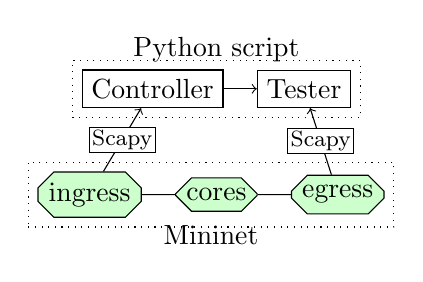
\begin{tikzpicture}[
        outer sep=auto,
        every node/.style={draw, rectangle, label distance=-4pt},
        switch/.style={chamfered rectangle, fill=green!20, inner sep=1pt},
        % every fit/.style={rectangle,draw}
    ]
        \node (controller) {Controller};
        \node[right=12pt of controller] (tester) {Tester};
        \draw[->] (controller) to (tester);
        \node[label=above:Python script, dotted,
          fit={(controller) (tester)}] (py) {};

        \node[switch, below=32pt] at (py) (s1) {cores};
        \node[switch, left=12pt] at (s1.west) (ingress) {ingress};
        \node[switch, right=12pt] at (s1.east)      (egress) {egress};
        \draw (ingress) to (s1);
        \draw (s1) to (egress);
        \node[label=below:Mininet, dotted,
            fit={(ingress) (s1) (egress)}] {};

        \draw[->] (ingress) -- node[fill=white, inner sep=1pt] {\footnotesize Scapy} (controller);
        \draw[->] (egress) -- node[fill=white, inner sep=1pt] {\footnotesize Scapy} (tester) ;
    \end{tikzpicture}
    \caption{Experimentation setup}
    \label{setup}
    \end{minipage}
    \begin{minipage}{0.49\linewidth}
    \centering    
    \newcommand{\nodescale}{0.8}
    \newcommand{\nswitches}{10}
    % with ports
    % \newcommand{\hspacing}{0.95}
    % \newcommand{\vspacing}{0.95}
    % \newcommand{\nodescale}{0.8}
    % \newcommand{\nswitches}{10}
    % \begin{tikzpicture}[outer sep=auto]
    %     \foreach \x in {1, ..., \nswitches} {
    %         \node[host] (H\x) at (\x*\hspacing, 0*\vspacing) {$h\x$};
    %         \node[edge] (E\x) at (\x*\hspacing, 0.95*\vspacing) {$e\x$};
    %         \node[core] (S\x) at (\x*\hspacing, 2*\vspacing) {$s\x$};

    %         \draw (H\x) to
    %             node[pos=0.1, port, signal to=north]{1}
    %             node[pos=0.9, port, signal to=south]{1}
    %             (E\x);
    %         \draw (E\x) to
    %             node[pos=0.1, port, signal to=north]{2}
    %             node[pos=0.9, port, signal to=south]{1}
    %             (S\x);
    %     };
    %     \node[host] (H11) at (0*\hspacing, 0*\vspacing) {$h11$};
    %     \draw (H11) to
    %         node[pos=0.1, port, signal to=north]{1}
    %         node[pos=0.9, port, signal to=south]{3}
    %         (E1);
        
    %     \draw (S1) to
    %         node[pos=-0.1, port, signal to=right]{2}
    %         node[pos=1.1, port, signal to=left]{2}
    %         (S2);
    %     \foreach \x in {2, ...,  \number\numexpr\nswitches-1\relax } {
    %         \draw (S\x) to
    %             node[pos=-0.1, port, signal to=right]{3}
    %             node[pos=1.1, port, signal to=left]{2}
    %             (S\number\numexpr\x+ 1\relax);
    %     };
            
    % \end{tikzpicture}

    % Without ports

    \newcommand{\newtopoitem}[2]{%
        \node[host, right=2pt] (H#1) at (H#2.east)  {$h_{#1}$};
        \node[edge, above=4pt] (E#1) at (H#1.north) {$e_{#1}$};
        \node[core, above=4pt] (S#1) at (E#1.north) {$s_{#1}$};
        \draw (H#1) -- (E#1) -- (S#1);
    }
    \setcounter{previtem}{11}
    \begin{tikzpicture}[outer sep=auto]
        \node[host] (H11) {$h_11$};
        \foreach \x in {1, ..., \nswitches} {
            \newtopoitem{\x}{\arabic{previtem}}
            \ifnum \theprevitem < 11
                \draw (S\x) to (S\theprevitem);
            \fi
            \setcounter{previtem}{\x}
        };
        \draw (H11) to (E1);
            
    \end{tikzpicture}
    \caption{Baseline topology used in experimentation}
    \label{topology:base}
    \end{minipage}
% \end{figure}
% Joins both figures into one
% \begin{figure}[ht]
%     \centering
    \tikzset{
        outer sep=auto,
        every node/.style={draw, chamfered rectangle, label distance=-4pt, inner sep=2pt},
    }
    \begin{minipage}{0.49\linewidth}
    \centering    
    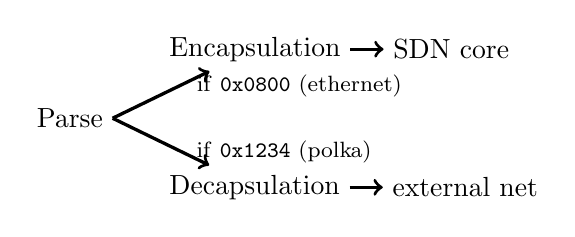
\begin{tikzpicture}
        \node (parse) {Parse};
            
        \node[above right=24pt] (encap) at (parse.east) {Encapsulation};
        \node[right=12pt] (core) at (encap.east) {SDN core};
        \draw[->, very thick] (parse.east) -- (encap)
            node[draw=none,pos=0.7,xshift=2pt,anchor=mid west] {\footnotesize if \texttt{0x0800} (ethernet)};
        \draw[->, very thick] (encap) -- (core);
        
        \node[below right=24pt] (decap) at (parse.east) {Decapsulation};
        \node[right=12pt] (out) at (decap.east) {external net};
        \draw[->, very thick] (parse.east) -- (decap)
            node[draw=none,pos=0.7,xshift=2pt, anchor=mid west] {\footnotesize if \texttt{0x1234} (polka)};
        \draw[->, very thick] (decap) -- (out);
    \end{tikzpicture}
    \caption{Edge ingress/egress steps}
    \label{fig:pipeline-edge}
    \end{minipage}
    \begin{minipage}{0.49\linewidth}
    \centering    
    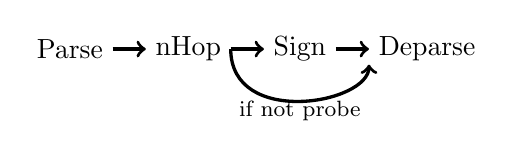
\begin{tikzpicture}
        \node (parse) {Parse};
        \node[right=12pt] (nhop) at (parse.east) {nHop};
        \node[right=12pt] (sign) at (nhop.east) {Sign};
        \node[right=12pt] (deparse) at (sign.east) {Deparse};

        \draw[->, very thick] (parse) -- (nhop);
        \draw[->, very thick] (nhop) -- (sign);
        \draw[->, very thick] 
            (nhop.east) ..controls ++(0,-1) and ++(0,-0.5) .. (deparse.195) node[midway,below=-4pt,draw=none] {\footnotesize if not probe};
        \draw[->, very thick] (sign) -- (deparse);
            
    \end{tikzpicture}
    \caption{Data plane steps \mycomment{Muito simples?}}
    \label{fig:pipeline-core}
    \end{minipage}
\end{figure}

On edge nodes, if an IPv4 protocol \texttt{ethertype} field is detected (\texttt{0x0800}), it must be a packet from outside the network, so the edge is doing an ingress and \polka headers need to be added. Let this process be called \textit{encapsulation}; If a \polka protocol \texttt{ethertype} field is detected (\texttt{0x1234}), it must be a packet from the network core, so the edge is doing an egress and the original IPv4 packet must be unwrapped. Let this process be called \textit{decapsulation}.

\polka headers consists of the route polynomial (\routeid), along with \texttt{version}, \texttt{ttl} and \texttt{proto} (stores the original \texttt{ethertype}). \routeid and hop calculation is out of the scope of this paper.
During encapsulation, the packet can be made into a probe packet by setting the \texttt{version} header field to \texttt{0xF1} and further defining the 32-bit fields \timestamp to any unique value and \lhash to \timestamp.

On the core network, the hash function used is \textit{SipHash-2-4-32} (\siphash), which after calculating the next hop (\nhop) and if the packet is a probe packet \lhash is computed as
$$
\lhash \leftarrow \textit{SipHash2-4-32}(\nodeid || \nhop || \timestamp || 0000000_2, \lhash)
$$
Meaning that a 64-bitstring made of concatenating \nodeid, \nhop, \timestamp and 7 bit wide zero is used as key for the \siphash function hashing \lhash. Inputting \nhop into the hash function protects us from some scenarios. \mycomment{explicar mais}


\section{Adversity scenarios}

\mycommentbox{
- explica no 1o paragraf. que nesta sec. vc vai apresentar os testes representando diferente cenenários de falha/ataque

- CRIAR UMA FIGURONA, colocando as 4 fig juntas (faz um sub tit de fig (a), (b), etc)

um tabelão pra todos os cenários

}

This section presents results for various tests representing different adversity scenarios. Each scenario is designed to evaluate the robustness and security of the system under specific attack or misconfiguration conditions. The scenarios include addition, detour, skipping, and out-of-order packet delivery. \autoref{tab:adversity_checksums} shows 
the checksums for each scenario, highlighting the differences caused by the adversarial conditions. Note that a scenario may result in a different amount of hashes to compare (e.g. addition), so the table appears to be missing cells. For all of the scenario, a ping from $h_1$ to $h_{10}$ was performed, resulting in \routeid = \texttt{0x707b3a1d61d1d0d8b9fc91e442d0360dfc8bba4}.

\begin{table}
    \newcommand{\red}{\cellcolor{red!50}}
    \centering
    \scriptsize
    \begin{tabularx}{\linewidth}{ll|ll|ll|ll|ll}
        \hline
        \multicolumn{2}{c|}{\small Reference} & \multicolumn{2}{c|}{\small Addition} & \multicolumn{2}{c|}{\small Detour} & \multicolumn{2}{c|}{\small Skipping} & \multicolumn{2}{c}{\small Out-of-order} \\
         \hline
         \hline%                                Add                                      DET                             SKP                          OOO
         seed    &\texttt{0x61e8d6e7}&seed         &\texttt{0x61e8d6e7}    &seed         &\texttt{0x61e8d6e7}    &seed        &\texttt{0x61e8d6e7}    &seed         &\texttt{0x61e8d6e7} \\
         $s_1$   &\texttt{0xd25dc935}&$s_1$        &\texttt{0xd25dc935}    &$s_1$        &\texttt{0xd25dc935}    &$s_1$       &\texttt{0xd25dc935}    &$s_1$        &\texttt{0xd25dc935} \\
         $s_2$   &\texttt{0x245b7ac5}&$s_2$        &\texttt{0x245b7ac5}    &$s_2$        &\texttt{0x245b7ac5}    &$s_2$       &\texttt{0x245b7ac5}    &$s_2$        &\texttt{0x245b7ac5} \\
         $s_3$   &\texttt{0xa3b38b83}&$s_3$        &\texttt{0xa3b38b83}    &$s_3$        &\texttt{0xa3b38b83}    &$s_3$       &\texttt{0xa3b38b83}    &$s_3$        &\texttt{0xa3b38b83} \\
         $s_4$   &\texttt{0x26aee736}&$s_4$        &\texttt{0x26aee736}    &$s_4$        &\texttt{0x26aee736}    &$s_4$       &\texttt{0x26aee736}    &$s_4$        &\texttt{0x26aee736} \\
         $s_5$   &\texttt{0xf9b47914}&$s_5$        &\texttt{0xf9b47914}    &$s_5$        &\texttt{0xf9b47914}    &            &                       &             &                    \\
                 &                   &\red$s_{add}$&\red\texttt{0x18c6d8d1}&             &                       &            &                       &\red$s_6$    &\red\texttt{0x4b5a6c5a} \\
         $s_6$   &\texttt{0x18c6d8d1}&\red$s_6$    &\red\texttt{0xb69b99ec}&\red$s_{det}$&\red\texttt{0x250822a2}&\red$s_6$   &\red\texttt{0x4b5a6c5a}&\red$s_5$    &\red\texttt{0xde3862a0} \\
         $s_7$   &\texttt{0xb69b99ec}&\red$s_7$    &\red\texttt{0xfe6117f8}&\red$s_7$    &\red\texttt{0x40298bb9}&\red$s_7$   &\red\texttt{0x002346d3}&\red$s_7$    &\red\texttt{0x648556ec} \\
         $s_8$   &\texttt{0xfe6117f8}&\red$s_8$    &\red\texttt{0xc8d9fbde}&\red$s_8$    &\red\texttt{0xe13dcc9b}&\red$s_8$   &\red\texttt{0x7ec711aa}&\red$s_8$    &\red\texttt{0x144e1d1b} \\
         $s_9$   &\texttt{0xc8d9fbde}&\red$s_9$    &\red\texttt{0xa6293a25}&\red$s_9$    &\red\texttt{0x1bf62c19}&\red$s_9$   &\red\texttt{0x5ee32b7b}&\red$s_9$    &\red\texttt{0x9e818f34} \\
         \hline
         $s_{10}$&\texttt{0xa6293a25}&\red$s_{10}$ &\red\texttt{0xf4bcdf07}&\red$s_{10}$ &\red\texttt{0xdd3a6675}&\red$s_{10}$&\red\texttt{0xc973a219}&\red$s_{10}$ &\red\texttt{0x6f694bc} \\
         \hline
         \hline
    \end{tabularx}
    \caption{Intermediary \lhash for different test scenarios with the same seed}
    \label{tab:adversity_checksums}
\end{table}

\begin{figure}[h]
    \centering
    \tikzset{
        host/.style={
            scale=\nodescale,
            inner sep=1pt,
            draw,
            rounded rectangle,
        },
        edge/.style={
            scale=\nodescale,
            inner sep=1pt,
            draw,
            rounded rectangle,
            fill=blue!20,
        },
        core/.style={
            scale=\nodescale,
            inner sep=1pt,
            draw,
            rounded rectangle,
            fill=green!30,
        },
        port/.style = {
            % font=\tiny,
            scale=.5,
            inner sep=1pt,
            draw,
            signal,
            fill=white,
        }
        }

    \newcommand{\nodescale}{0.8}
    \newcommand{\nswitches}{10}
    \newcommand{\newtopoitem}[2]{%
        \node[host, right=2pt] (H#1) at (H#2.east)  {$h_{#1}$};
        \node[edge, above=4pt] (E#1) at (H#1.north) {$e_{#1}$};
        \node[core, above=4pt] (S#1) at (E#1.north) {$s_{#1}$};
        \draw (H#1) -- (E#1) -- (S#1);
    }
    \newcommand{\newtopoitemanchors}[2]{%
        \node[core, below right=4pt] (S#1) at (#2.east)   {$s_{#1}$};
        \node[edge, below=4pt] (E#1) at (S#1.south) {$e_{#1}$};
        \node[host, below=4pt] (H#1) at (E#1.south) {$h_{#1}$};
        \draw (H#1) -- (E#1) -- (S#1);
    }
    \begin{subfigure}[t]{0.49\linewidth}
        \centering
        \newcommand{\splitpoint}{5} %switch is added after s5
        \setcounter{previtem}{11}
        \begin{tikzpicture}[outer sep=auto]
            \node[host] (H11) {$h_{11}$};
            \foreach \x in {1, ..., \splitpoint} {
                \newtopoitem{\x}{\arabic{previtem}}
                \ifnum \theprevitem < 11
                    \draw (S\x) to (S\theprevitem);
                \fi
                \setcounter{previtem}{\x}
            };
            \draw (H11) to (E1);

            \node[core, above right=4pt] at (S\theprevitem.east) (Sadd) {$s_{add}$};
            \newtopoitemanchors{6}{Sadd}
            \draw (S5) -- (Sadd) -- (S6);
            \stepcounter{previtem}

            \foreach \x in {\number\numexpr\splitpoint+2\relax, ..., \nswitches} {
                \newtopoitem{\x}{\arabic{previtem}}
                \draw (S\x) to (S\theprevitem);
                \setcounter{previtem}{\x}
            };
                
        \end{tikzpicture}
        \caption{Addition}
        \label{topology:addition}
    \end{subfigure}
    \begin{subfigure}[t]{0.49\linewidth}
        \centering
        \newcommand{\splitpoint}{5} %switch is removed after s5
        \setcounter{previtem}{11}
        \begin{tikzpicture}[outer sep=auto]
            \node[host] (H11) {$h_{11}$};
            \foreach \x in {1,2,3,4,6,7,8,9,10} {
                \newtopoitem{\x}{\arabic{previtem}}
                \ifnum \theprevitem < 11
                    \draw (S\x) to (S\theprevitem);
                \fi
                \setcounter{previtem}{\x}
            };
            \draw (H11) to (E1);
                
        \end{tikzpicture}
        \caption{Skipping}
        \label{topology:skipping}
    \end{subfigure}

    \begin{subfigure}{0.49\linewidth}
        \centering
        \newcommand{\splitpoint}{5} %switch is detoured after s5
        \setcounter{previtem}{11}
        \begin{tikzpicture}[outer sep=auto]
            \node[host] (H11) {$h_{11}$};
            \foreach \x in {1,...,\nswitches} {
                \newtopoitem{\x}{\arabic{previtem}}
                \ifnum \theprevitem < 11
                    \draw (S\x) to (S\theprevitem);
                \fi
                \setcounter{previtem}{\x}
            };
            \draw (H11) to (E1);

            \node[core, above=2pt, anchor=south] at (S6.north) (Sdet) {$s_{det}$};
            \draw (S5) -- (Sdet) -- (S7);
                
        \end{tikzpicture}
        \caption{Detour}
        \label{topology:detour}
    \end{subfigure}
    \begin{subfigure}{0.49\linewidth}
        \centering
        \newcommand{\splitpoint}{5} %switch is changed after s5
        \setcounter{previtem}{11}
        \begin{tikzpicture}[outer sep=auto]
            \node[host] (H11) {$h_{11}$};
            \foreach \x in {1,2,3,4,6,5,7,8,9,10} {
                \newtopoitem{\x}{\arabic{previtem}}
                \ifnum \theprevitem < 11
                    \draw (S\x) to (S\theprevitem);
                \fi
                \setcounter{previtem}{\x}
            };
            \draw (H11) to (E1);                
        \end{tikzpicture}
        \caption{Out of order}
        \label{topology:outoforder}
    \end{subfigure}

    \caption{Topologies for tested scenarios}
    \label{fig:topologies}
\end{figure}

The solution has been tested against some adversarial scenarios, and checked against the same initial seed but under the base topology as described on \ref{topology:base}.

%attack model


\subsection{Addition} \label{scenario:addition}

An attacker PolKA switch $s_{555}$ was added between $s_5$ and $s_6$, as shown in \ref{topology:addition}. The packet was sent from $e_1$ to $e_{10}$. Suppose the attacking switch is properly connected in the ports that PolKA uses for this route, the packet is properly routed with PolKA. The checksums will not match when validating the path past the attacker. The packet trace is shown in \ref{example:addition}. Note the error propagating nature of composing checksums.

\mycommentbox{FIGURA}
% #figure(
%   caption: [Topology setup for addition scenario.],
%   diagram(
%       // debug: 1,
%       spacing: 2em,
%       label-size: 6pt,
%       label-sep: 2pt,
%       {

%       let node_base = node.with(stroke: 0.5pt, inset: 4pt)
%       let switch = node_base.with(shape: shapes.octagon, fill: aqua)
%       let edge_router = node_base.with(shape: shapes.pill, fill: lime)
%       let host = node_base.with(shape: shapes.rect, fill: yellow, inset: 3.5pt)
%         let first_1 = 1
%         let last_1 = 10
%         for i in range(first_1, last_1+1) {
%           let s = "s" + str(i)
%           switch((i, 0), name: label(s))[$s_#i$]
%           if i > first_1 and i != 6 {
%             if i == 2 {
%               edge(label("s" + str(i - 1)), label("s" + str(i)), "<->", 1, label-pos: 0.2)
%             } else {
%               edge(label("s" + str(i - 1)), label("s" + str(i)), "<->", 2, label-pos: 0.2)
%             }
%             edge(label("s" + str(i - 1)), label("s" + str(i)), "<->", 1, label-pos: 0.8)
%           }
%           edge("<->", label-pos: 0.2, label-side: left, label: 0)
%           let e = "e" + str(i)
%           edge_router((rel: (0, 1)), name: label(e))[$e_#i$]
%           if i > first_1 {
%             let h = "h" + str(i)
%             edge("<->")
%             host((rel: (0, 1)), name: label(h))[$h_#i$]
%           }
%         }


%         host((rel: (-0.3, 1), to: <e1>), name: <h1>)[$h_1$]
%         edge("<->", <e1>)
%         host((rel: (0.3, 1), to: <e1>), name: <h11>)[$h_11$]
%         edge("<->", <e1>)

%         switch((rel: (0, -1), to:(<s5>, 50%, <s6>)), name: <s555>)[$s_555$]
%         edge("<->", <s5>, 2, label-pos: 0.8)
%         edge("<->", <s5>, 0, label-pos: 0.3)
%         edge("<->", <s6>, 1, label-pos: 0.8)
%         edge("<->", <s6>, 1, label-pos: 0.3)
%         },
%       ),
% ) <topology:addition>


% #figure(
%   caption: [Packet trace while traversing $limits(P)_(e_1->e_10)$ with an unexpected addition $s_555$.],
%   table(
%       columns: 6,
%       table.header(
%         [Node],
%         [`node_id`],
%         [`exit_port`],
%         [Calculation],
%         [`l_hash`],
%         [Expected],
%       ),

%       /*
%       *** Comparing 0xabadcafe, expects 0xabadcafe on node 0x00ff:e1-eth2 ✅ ok
%       *** Comparing 0xabadcafe, expects 0xabadcafe on node 0x00ff:s1-eth1 ✅ ok
%       *** Comparing 0x432cf798, expects 0x432cf798 on node 0x002b:s1-eth2 ✅ ok
%       *** Comparing 0x432cf798, expects 0x432cf798 on node 0x002b:s2-eth2 ✅ ok
%       *** Comparing 0xe04df688, expects 0xe04df688 on node 0x002d:s2-eth3 ✅ ok
%       *** Comparing 0xe04df688, expects 0xe04df688 on node 0x002d:s3-eth2 ✅ ok
%       *** Comparing 0xe8f0142c, expects 0xe8f0142c on node 0x0039:s3-eth3 ✅ ok
%       *** Comparing 0xe8f0142c, expects 0xe8f0142c on node 0x0039:s4-eth2 ✅ ok
%       *** Comparing 0xb452022a, expects 0xb452022a on node 0x003f:s4-eth3 ✅ ok
%       *** Comparing 0xb452022a, expects 0xb452022a on node 0x003f:s5-eth2 ✅ ok
%       *** Comparing 0x4450d2d2, expects 0x4450d2d2 on node 0x0047:s5-eth3 ✅ ok
%       *** Comparing 0x4450d2d2, expects 0x4450d2d2 on node 0x0047:s555-eth0 ✅ ok
%       *** Comparing 0x5b0fce3e, expects 0xe9367b57 on node 0x0047:s555-eth1 ❌ Digest does not match
%       *** Comparing 0x5b0fce3e, expects 0xe9367b57 on node 0x0047:s6-eth4 ❌ Digest does not match
%       *** Comparing 0xc967a61d, expects 0x991182c1 on node 0x0053:s6-eth3 ❌ Digest does not match
%       *** Comparing 0xc967a61d, expects 0x991182c1 on node 0x0053:s7-eth2 ❌ Digest does not match
%       *** Comparing 0xf6c27aa4, expects 0x35e72e11 on node 0x008d:s7-eth3 ❌ Digest does not match
%       *** Comparing 0xf6c27aa4, expects 0x35e72e11 on node 0x008d:s8-eth2 ❌ Digest does not match
%       *** Comparing 0x38d0bc4f, expects 0xaa152eb9 on node 0x00bd:s8-eth3 ❌ Digest does not match
%       *** Comparing 0x38d0bc4f, expects 0xaa152eb9 on node 0x00bd:s9-eth2 ❌ Digest does not match
%       *** Comparing 0xb6ff911a, expects 0x1a1573e7 on node 0x00d7:s9-eth3 ❌ Digest does not match
%       *** Comparing 0xb6ff911a, expects 0x1a1573e7 on node 0x00d7:s10-eth2 ❌ Digest does not match
%       *** ❌ Route length does not match expected. Expected 22, got 24
%       *** ❌ Leftover packets:
%       *** 0x882d8e93 on node 0x00f5:s10-eth1
%       *** 0x882d8e93 on node 0x00f5:e10-eth2
%       */

%       ..green_cells(
%         $e_1$, ""         , `1` , [Generation]                      , `0xabadcafe`, `0xabadcafe`,
%         $s_1$, `0x002b`   , `1` , calc_crc32(0xabadcafe, 1, 0x002b) , `0x432cf798`, `0x432cf798`,
%         $s_2$, `0x002d`   , `2` , calc_crc32(0x432cf798, 2, 0x002d) , `0xe04df688`, `0xe04df688`,
%         $s_3$, `0x0039`   , `2` , calc_crc32(0xe04df688, 2, 0x0039) , `0xe8f0142c`, `0xe8f0142c`,
%         $s_4$, `0x003f`   , `2` , calc_crc32(0xe8f0142c, 2, 0x003f) , `0xb452022a`, `0xb452022a`,
%         $s_5$, `0x0047`   , `2` , calc_crc32(0xb452022a, 2, 0x0047) , `0x4450d2d2`, `0x4450d2d2`
%       ),
%       ..red_cells(
%         $s_555$, `0x0047` , `1` , calc_crc32(0x4450d2d2, 1, 0x0047) , `0x5b0fce3e`, ""          ,
%         $s_6$, `0x0053`   , `2` , calc_crc32(0x5b0fce3e, 2, 0x0053) , `0xc967a61d`, `0xe9367b57`,
%         $s_7$, `0x008d`   , `2` , calc_crc32(0xc967a61d, 2, 0x008d) , `0xf6c27aa4`, `0x991182c1`,
%         $s_8$, `0x00bd`   , `2` , calc_crc32(0xf6c27aa4, 2, 0x00bd) , `0x38d0bc4f`, `0x35e72e11`,
%         $s_9$, `0x00d7`   , `2` , calc_crc32(0x38d0bc4f, 2, 0x00d7) , `0xb6ff911a`, `0xaa152eb9`,
%         $s_10$, `0x00f5`  , `0` , calc_crc32(0xb6ff911a, 0, 0x00f5) , `0x882d8e93`, `0x1a1573e7`,
%         $e_10$, ""        , `0` , [Decapsulation]                   , `0x882d8e93`, `0x1a1573e7`
%       ),
%     ),
% ) <example:addition>

\subsection{Detour} \label{scenario:detour}

An attacker tries to make a detour in the network, as shown in \ref{topology:detour}. The packet was sent from $e_1$ to $e_{10}$, and passed through the detour, as shown in \ref{example:detour}. The checksum will fail to validate when checking in the futures, as the function composition $f_{s_{555}} (x) = f_{s_6} (x)$. Note that this is only true when $k_{s_{555}} \neq k_{s_6}$. As stated, the key must be unique per node, and so must be kept secret.

\mycommentbox{FIGURA}
% #figure(
%   caption: [Topology setup for detour scenario.],
%   diagram(
%       // debug: 1,
%       spacing: 2em,
%       label-size: 6pt,
%       label-sep: 2pt,
%       {

%       let node_base = node.with(stroke: 0.5pt, inset: 4pt)
%       let switch = node_base.with(shape: shapes.octagon, fill: aqua)
%       let edge_router = node_base.with(shape: shapes.pill, fill: lime)
%       let host = node_base.with(shape: shapes.rect, fill: yellow, inset: 3.5pt)
%         let first_1 = 1
%         let last_1 = 10
%         for i in range(first_1, last_1+1) {
%           let s = "s" + str(i)
%           switch((i, 0), name: label(s))[$s_#i$]
%           if i > first_1 and i not in (6,7) {
%             if i == 2 {
%               edge(label("s" + str(i - 1)), label("s" + str(i)), "<->", 1, label-pos: 0.2)
%             } else {
%               edge(label("s" + str(i - 1)), label("s" + str(i)), "<->", 2, label-pos: 0.2)
%             }
%             edge(label("s" + str(i - 1)), label("s" + str(i)), "<->", 1, label-pos: 0.8)
%           }
%           edge("<->", label-pos: 0.2, label-side: left, label: 0)
%           let e = "e" + str(i)
%           edge_router((rel: (0, 1)), name: label(e))[$e_#i$]
%           if i > first_1 {
%             let h = "h" + str(i)
%             edge("<->")
%             host((rel: (0, 1)), name: label(h))[$h_#i$]
%           }
%         }


%         host((rel: (-0.3, 1), to: <e1>), name: <h1>)[$h_1$]
%         edge("<->", <e1>)
%         host((rel: (0.3, 1), to: <e1>), name: <h11>)[$h_11$]
%         edge("<->", <e1>)

%         switch((rel: (0, -1), to:(<s5>, 50%, <s7>)), name: <s555>)[$s_555$]
%         edge("<-o", <s5>, label-pos: 0.2, 0)
%         edge("<-o", <s5>, label-pos: 0.8, 2)
%         edge("o->", <s7>, label-pos: 0.2, 1)
%         edge("o->", <s7>, label-pos: 0.8, 3)
%         edge(<s5>, "<-o", <s6>, label-pos: 0.8, 1)
%         edge(<s6>, "<-o", <s7>, label-pos: 0.8, 1)
%         },
%       ),
% ) <topology:detour>

% #figure(
%   caption: [Packet trace while traversing $limits(P)_(e_1->e_10)$ with an unexpected detour.],
%   table(
%       columns: 6,
%       table.header(
%         [Node],
%         [`node_id`],
%         [`exit_port`],
%         [Calculation],
%         [`l_hash`],
%         [Expected]
%       ),

%       /*
%       *** Comparing 0xbaddc0de, expects 0xbaddc0de on node 0x00ff:e1-eth2 ✅ ok
%       *** Comparing 0xbaddc0de, expects 0xbaddc0de on node 0x00ff:s1-eth1 ✅ ok
%       *** Comparing 0x3ef96770, expects 0x3ef96770 on node 0x002b:s1-eth2 ✅ ok
%       *** Comparing 0x3ef96770, expects 0x3ef96770 on node 0x002b:s2-eth2 ✅ ok
%       *** Comparing 0x2dca9942, expects 0x2dca9942 on node 0x002d:s2-eth3 ✅ ok
%       *** Comparing 0x2dca9942, expects 0x2dca9942 on node 0x002d:s3-eth2 ✅ ok
%       *** Comparing 0x11797334, expects 0x11797334 on node 0x0039:s3-eth3 ✅ ok
%       *** Comparing 0x11797334, expects 0x11797334 on node 0x0039:s4-eth2 ✅ ok
%       *** Comparing 0x98081e3e, expects 0x98081e3e on node 0x003f:s4-eth3 ✅ ok
%       *** Comparing 0x98081e3e, expects 0x98081e3e on node 0x003f:s5-eth2 ✅ ok
%       *** Comparing 0x3332e012, expects 0x3332e012 on node 0x0047:s5-eth3 ✅ ok
%       *** Comparing 0x3332e012, expects 0x3332e012 on node 0x0047:s555-eth0 ✅ ok
%       *** Comparing 0x90a0df94, expects 0x22996afd on node 0x0047:s555-eth1 ❌ Digest does not match
%       *** Comparing 0x90a0df94, expects 0x22996afd on node 0x0047:s7-eth2 ❌ Digest does not match
%       *** Comparing 0xbebe4372, expects 0x8fa3987d on node 0x008d:s7-eth3 ❌ Digest does not match
%       *** Comparing 0xbebe4372, expects 0x8fa3987d on node 0x008d:s8-eth2 ❌ Digest does not match
%       *** Comparing 0x5aafa7f2, expects 0xf4b50950 on node 0x00bd:s8-eth3 ❌ Digest does not match
%       *** Comparing 0x5aafa7f2, expects 0xf4b50950 on node 0x00bd:s9-eth2 ❌ Digest does not match
%       *** Comparing 0x649b8554, expects 0xd0c29e67 on node 0x00d7:s9-eth3 ❌ Digest does not match
%       *** Comparing 0x649b8554, expects 0xd0c29e67 on node 0x00d7:s10-eth2 ❌ Digest does not match
%       *** Comparing 0xf46427bf, expects 0x13ff41c1 on node 0x00f5:s10-eth1 ❌ Digest does not match
%       *** Comparing 0xf46427bf, expects 0x13ff41c1 on node 0x00f5:e10-eth2 ❌ Digest does not match
%       */

%       ..green_cells(
%         $e_1$, ""         , `1` , [Generation]                      , `0xbaddc0de`, `0xbaddc0de`,
%         $s_1$, `0x002b`   , `1` , calc_crc32(0xbaddc0de, 1, 0x002b) , `0x3ef96770`, `0x3ef96770`,
%         $s_2$, `0x002d`   , `2` , calc_crc32(0x3ef96770, 2, 0x002d) , `0x2dca9942`, `0x2dca9942`,
%         $s_3$, `0x0039`   , `2` , calc_crc32(0x2dca9942, 2, 0x0039) , `0x11797334`, `0x11797334`,
%         $s_4$, `0x003f`   , `2` , calc_crc32(0x11797334, 2, 0x003f) , `0x98081e3e`, `0x98081e3e`,
%         $s_5$, `0x0047`   , `2` , calc_crc32(0x98081e3e, 2, 0x0047) , `0x3332e012`, `0x3332e012`
%       ),
%       ..red_cells(
%         $s_555$, `0x0047` , `1` , calc_crc32(0x3332e012, 1, 0x0047) , `0x90a0df94`, `0x22996afd`,
%         $s_7$, `0x0053`   , `2` , calc_crc32(0x90a0df94, 2, 0x0053) , `0xbebe4372`, `0x8fa3987d`,
%         $s_8$, `0x008d`   , `2` , calc_crc32(0xbebe4372, 2, 0x008d) , `0x5aafa7f2`, `0xf4b50950`,
%         $s_9$, `0x00bd`   , `2` , calc_crc32(0x5aafa7f2, 2, 0x00bd) , `0x649b8554`, `0xd0c29e67`,
%         $s_10$, `0x00d7`  , `0` , calc_crc32(0x649b8554, 2, 0x00d7) , `0xf46427bf`, `0x13ff41c1`,
%         $e_10$, ""        , `0` , [Decapsulation]                   , `0xf46427bf`, `0x13ff41c1`
%       ),
%     ),
% ) <example:detour>

\subsection{Skipping} \label{scenario:skipping}

Misconfigured links can cause packets to skip nodes, as shown in \ref{topology:skipping}. The packet was sent from $e_1$ to $e_{10}$, and passed through the skipping, as shown in \ref{example:skipping}. The checksum will not match when validating the path in the future, as the packet did not pass through the expected nodes.

\mycommentbox{FIGURA}
% #figure(
%   caption: [Topology setup for skipping scenario.],
%   diagram(
%       // debug: 1,
%       spacing: 2em,
%       label-size: 6pt,
%       label-sep: 2pt,
%       {

%       let node_base = node.with(stroke: 0.5pt, inset: 4pt)
%       let switch = node_base.with(shape: shapes.octagon, fill: aqua)
%       let edge_router = node_base.with(shape: shapes.pill, fill: lime)
%       let host = node_base.with(shape: shapes.rect, fill: yellow, inset: 3.5pt)
%         let first_1 = 1
%         let last_1 = 10
%         for i in range(first_1, last_1+1) {
%           let s = "s" + str(i)
%           switch((i, 0), name: label(s))[$s_#i$]
%           if i > first_1 and i not in (5,6,) {
%             if i == 2 {
%               edge(label("s" + str(i - 1)), label("s" + str(i)), "<->", 1, label-pos: 0.2)
%             } else {
%               edge(label("s" + str(i - 1)), label("s" + str(i)), "<->", 2, label-pos: 0.2)
%             }
%             edge(label("s" + str(i - 1)), label("s" + str(i)), "<->", 1, label-pos: 0.8)
%           }
%           edge("<->", label-pos: 0.2, label-side: left, label: 0)
%           let e = "e" + str(i)
%           edge_router((rel: (0, 1)), name: label(e))[$e_#i$]
%           if i > first_1 {
%             let h = "h" + str(i)
%             edge("<->")
%             host((rel: (0, 1)), name: label(h))[$h_#i$]
%           }
%         }


%         host((rel: (-0.3, 1), to: <e1>), name: <h1>)[$h_1$]
%         edge("<->", <e1>)
%         host((rel: (0.3, 1), to: <e1>), name: <h11>)[$h_11$]
%         edge("<->", <e1>)


%         edge(<s4>, <s6>, "<->", 2, bend: 30deg, label-pos: 0.2)
%         edge(<s4>, <s6>, "<->", 1, bend: 30deg, label-pos: 0.8)
%         },
%       ),
% ) <topology:skipping>

% #figure(
%   caption: [Packet trace while traversing $limits(P)_(e_1->e_10)$ with an unexpected skip.],
%   table(
%       columns: 6,
%       table.header(
%         [Node],
%         [`node_id`],
%         [`exit_port`],
%         [Calculation],
%         [`l_hash`],
%         [Expected]
%       ),

%       /*
%       *** �� Tracing new route
%       *** Comparing 0x61e8d6e7, expects 0x61e8d6e7 on node 0x00ff:e1-eth2 ✅ ok
%       *** Comparing 0x61e8d6e7, expects 0x61e8d6e7 on node 0x00ff:s1-eth1 ✅ ok
%       *** Comparing 0xae91434c, expects 0xae91434c on node 0x002b:s1-eth2 ✅ ok
%       *** Comparing 0xae91434c, expects 0xae91434c on node 0x002b:s2-eth2 ✅ ok
%       *** Comparing 0x08c97f5f, expects 0x08c97f5f on node 0x002d:s2-eth3 ✅ ok
%       *** Comparing 0x08c97f5f, expects 0x08c97f5f on node 0x002d:s3-eth2 ✅ ok
%       *** Comparing 0xeff1aad2, expects 0xeff1aad2 on node 0x0039:s3-eth3 ✅ ok
%       *** Comparing 0xeff1aad2, expects 0xeff1aad2 on node 0x0039:s4-eth2 ✅ ok
%       *** Comparing 0x08040c89, expects 0x08040c89 on node 0x003f:s4-eth3 ✅ ok
%       *** Comparing 0x08040c89, expects 0x08040c89 on node 0x003f:s6-eth2 ✅ ok
%       *** Comparing 0xb0437a53, expects 0xaa99ae2e on node 0x0053:s6-eth3 ❌ Digest does not match
%       *** Comparing 0xb0437a53, expects 0xaa99ae2e on node 0x0053:s7-eth2 ❌ Digest does not match
%       *** Comparing 0x63589d0a, expects 0x7669685e on node 0x008d:s7-eth3 ❌ Digest does not match
%       *** Comparing 0x63589d0a, expects 0x7669685e on node 0x008d:s8-eth2 ❌ Digest does not match
%       *** Comparing 0x629b7b3b, expects 0x03e1e388 on node 0x00bd:s8-eth3 ❌ Digest does not match
%       *** Comparing 0x629b7b3b, expects 0x03e1e388 on node 0x00bd:s9-eth2 ❌ Digest does not match
%       *** Comparing 0xbd53e851, expects 0x2138ffd3 on node 0x00d7:s9-eth3 ❌ Digest does not match
%       *** Comparing 0xbd53e851, expects 0x2138ffd3 on node 0x00d7:s10-eth2 ❌ Digest does not match
%       *** Comparing 0x90bdf731, expects 0x1ef2cbbe on node 0x00f5:s10-eth1 ❌ Digest does not match
%       *** Comparing 0x90bdf731, expects 0x1ef2cbbe on node 0x00f5:e10-eth2 ❌ Digest does not match
%       */

%       ..green_cells(
%         $e_1$, ""         , `1` , [Generation]                      , `0x61e8d6e7`, `0x61e8d6e7`,
%         $s_1$, `0x002b`   , `1` , calc_crc32(0x61e8d6e7, 1, 0x002b) , `0xae91434c`, `0xae91434c`,
%         $s_2$, `0x002d`   , `2` , calc_crc32(0xae91434c, 2, 0x002d) , `0x08c97f5f`, `0x08c97f5f`,
%         $s_3$, `0x0039`   , `2` , calc_crc32(0x08c97f5f, 2, 0x0039) , `0xeff1aad2`, `0xeff1aad2`,
%         $s_4$, `0x003f`   , `2` , calc_crc32(0xeff1aad2, 2, 0x003f) , `0x08040c89`, `0x08040c89`
%       ),
%       ..red_cells(
%         $s_6$, `0x0053`   , `2` , calc_crc32(0x08040c89, 2, 0x0053) , `0xb0437a53`, `0xaa99ae2e`,
%         $s_7$, `0x008d`   , `2` , calc_crc32(0xb0437a53, 2, 0x008d) , `0x63589d0a`, `0x7669685e`,
%         $s_8$, `0x00bd`   , `2` , calc_crc32(0x63589d0a, 2, 0x00bd) , `0x629b7b3b`, `0x03e1e388`,
%         $s_9$, `0x00d7`   , `2` , calc_crc32(0x629b7b3b, 2, 0x00d7) , `0xbd53e851`, `0x2138ffd3`,
%         $s_10$, `0x00f5`  , `0` , calc_crc32(0xbd53e851, 0, 0x00f5) , `0x90bdf731`, `0x1ef2cbbe`,
%         $e_10$, ""        , `0` , [Decapsulation]                   , `0x90bdf731`, `0x1ef2cbbe`
%       ),
%     ),
% ) <example:skipping>

\subsection{Out-of-order \colorbox{red}{TODO}} \label{scenario:outoforder}

\subsection{Discussion}]
\mycommentbox{
- limitações
    - recuperar dados do mininet
        - sair dados nativamente do switch
    - cenários que não resolvemos (replay, etc)
    - limite de escala do cryptoscheme -- é maior ou menor q o limite do Polka
    - tempo de cálculo do crypto line rate -- impossível de maneira realista no nosso setup atual (mininet)
    - dificuldade de programar e debugar (wireshark) em p4
    }

Upon developing the solution, a set of limitations were identified:
\begin{itemize}
    \item As with most cryptographic solutions, the system is only as secure as the key used. If the key is compromised, the entire system is compromised, since a malicious actor can easily generate the same checksums.
    \item Replay attack is undetectable if metadata is disconsidered. This is due to the switch entry port not being included in the validation, which allows an attacker to replay the packet from a different port.
\end{itemize}

\section{Conclusion and Future Work}

As the examples show, our solution is able to detect when a packet is not following the expected path for most cases, and can be used to detect misconfigurations in the network.

As next steps, more parts of \pathsec \cite{pathsec} could be easily integrated for proof-of-concept, as all necessary information is already readily collect to Python scripts, making it simple to create 
%BETA
a complete \pathsec
proof-of-concept software.

To improve the system for a real-world scenario, the ingress edge needs to relay the ingressed package metadata directly to the controller, and the egress edge will report the final checksum directly to the blockchain. Having it not passing through the controller.

Replay attacks are not detectable by the current solution, as the switch entry port is not included in the verification. This allows an attacker to replay a packet to a different port, and the system will accept it as a valid packet. Including the entry port in the checksum would also be an appreciable increase in security, since it increases the number of targets an attacker would need to breach at the same time to be able to alter the path. It could be included in the \siphash key, but a design decision is necessary: there are only 7 bits available, and the port number is 9 bits long. A possible solution would be to use the 8 least significant bits of the port number for both entry and exit port, limiting the number of ports checked before collision to 256, but this would be a reasonable trade-off for the increased security. So for a proof-of-concept, design was kept closed to the original \pathsec description.

An interesting work can be done to use a rotating key architecture to detect replay attacks. This is a difficult problem to solve, since the key must be rotated and shared in a way that does not break the network, and of course, a malicious actor cannot acquire it. The key must be shared between the nodes in a secure, atomic way to prevent the network to enter an irrecoverable state. \mycomment{Pareço estar me estendendo mto, mas ainda acho um problema interessante e queria anotar isso de alguma coisa. Mas é um problema buscando uma solução. Manter de alguma forma?}

Using a keyless hash function, or even a keyed one with hardcoded keys on deployment could be studied, as it would remove the need for a seed \timestamp, but it would require to be a cryptographic hash, otherwise the data used to hash (which needs to include at least the \nodeid) could be derived from a switch's output. This would open ways to use a faster cryptographic hash function, such as xxHash's XXH3.

A timing analysis and stress tests can both be done to check if the incurred overhead is acceptable for the network, but this would require it to be implemented in hardware, not only in Mininet. The overhead needs to be low 
%for it be
to represent a viable solution, otherwise the network will drop packets. Some overhead is acceptable since a configurable ratio/schedule of \polka packets are selected to be probe packets.

\mycomment{Acabou meio do nadão, não? Agora bateu um desespero}



\bibliographystyle{sbc}
\bibliography{bilbiography}

\end{document}
